\documentclass[10pt]{exam}

\usepackage{amssymb, amsmath, amsthm, mathrsfs, multicol, graphicx}
\usepackage{tikz}

 \def\d{\displaystyle}
\def\?{\reflectbox{?}}
\def\b#1{\mathbf{#1}}
\def\f#1{\mathfrak #1}
\def\c#1{\mathcal #1}
\def\s#1{\mathscr #1}
\def\r#1{\mathrm{#1}}
\def\N{\mathbb N}
\def\Z{\mathbb Z}
\def\Q{\mathbb Q}
\def\R{\mathbb R}
\def\C{\mathbb C}
\def\F{\mathbb F}
\def\A{\mathbb A}
\def\X{\mathbb X}
\def\E{\mathbb E}
\def\O{\mathbb O}
\def\U{\mathcal U}
\def\pow{\mathcal P}
\def\inv{^{-1}}
\def\nrml{\triangleleft}
\def\st{:}
\def\~{\widetilde}
\def\rem{\mathcal R}
\def\sigalg{$\sigma$-algebra }
\def\Gal{\mbox{Gal}}
\def\iff{\leftrightarrow}
\def\Iff{\Leftrightarrow}
\def\land{\wedge}
\def\And{\bigwedge}
\def\AAnd{\d\bigwedge\mkern-18mu\bigwedge}
\def\Vee{\bigvee}
\def\VVee{\d\Vee\mkern-18mu\Vee}
\def\imp{\rightarrow}
\def\Imp{\Rightarrow}
\def\Fi{\Leftarrow}

%\def\={\equiv}
\def\var{\mbox{var}}
\def\mod{\mbox{Mod}}
\def\Th{\mbox{Th}}
\def\sat{\mbox{Sat}}
\def\con{\mbox{Con}}
\def\bmodels{=\joinrel\mathrel|}
\def\iffmodels{\bmodels\models}
\def\dbland{\bigwedge \!\!\bigwedge}
\def\dom{\mbox{dom}}
\def\rng{\mbox{range}}
\DeclareMathOperator{\wgt}{wgt}


\def\bar{\overline}


\newcommand{\vtx}[2]{node[fill,circle,inner sep=0pt, minimum size=4pt,label=#1:#2]{}}
\newcommand{\va}[1]{\vtx{above}{#1}}
\newcommand{\vb}[1]{\vtx{below}{#1}}
\newcommand{\vr}[1]{\vtx{right}{#1}}
\newcommand{\vl}[1]{\vtx{left}{#1}}
\renewcommand{\v}{\vtx{above}{}}

\def\circleA{(-.5,0) circle (1)}
\def\circleAlabel{(-1.5,.6) node[above]{$A$}}
\def\circleB{(.5,0) circle (1)}
\def\circleBlabel{(1.5,.6) node[above]{$B$}}
\def\circleC{(0,-1) circle (1)}
\def\circleClabel{(.5,-2) node[right]{$C$}}
\def\twosetbox{(-2,-1.4) rectangle (2,1.4)}
\def\threesetbox{(-2.5,-2.4) rectangle (2.5,1.4)}
\newcommand{\twoline}[2]{\begin{pmatrix}#1 \\ #2 \end{pmatrix}}


\def\circleA{(-.5,0) circle (1)}
\def\circleAlabel{(-1.5,.6) node[above]{$A$}}
\def\circleB{(.5,0) circle (1)}
\def\circleBlabel{(1.5,.6) node[above]{$B$}}
\def\circleC{(0,-1) circle (1)}
\def\circleClabel{(.5,-2) node[right]{$C$}}
\def\twosetbox{(-2,-1.5) rectangle (2,1.5)}
\def\threesetbox{(-2,-2.5) rectangle (2,1.5)}

%\pointname{pts}
\pointsinmargin
\marginpointname{pts}
\addpoints
\pagestyle{head}
\printanswers

\firstpageheader{Math 228}{\bf Homework 6 Solutions}{Due: Wednesday, October 10}


\begin{document}
% \noindent \textbf{Instructions}: Same rules as usual.  Turn in solutions on separate pages, and do not consult the internet.

\begin{questions}


\question[8] We usually write numbers in decimal form (or base 10), meaning numbers are composed using 10 different ``digits'' $\{0,1,\ldots, 9\}$.  Sometimes though it is useful to write numbers in {\em hexadecimal} or base 16.  Now there are 16 distinct digits that can be used to form numbers: $\{0, 1, \ldots, 9, \mathrm{A, B, C, D, E, F}\}$.  So for example, a 3 digit hexadecimal number might be 3B8.
	\begin{parts}
	\part Write out all 2-digit hexadecimals are there in which the first digit is D, E, or F (you can you dot-dot-dots once the pattern is clear).  How many hexadecimals are in your list?  Explain how the additive principle works here.
		\begin{solution}
			D1, D2, \ldots, DF, E1, E2, \ldots, EF, F1, F2, \ldots, FF.

			There are 16 hexadecimals in which the first digit is an D (one for each choice of second digit).  Similarly, there are 16 hexadecimals in which the first digit is an E, and another 16 where the first digit is an F.  We want the union of these three disjoint sets, so there are $16 + 16 + 16 = 48$ two digits hexadecimals in our list.
		\end{solution}
	\part Explain how you can use the multiplicative principle to count the number of hexadecimals in the list as well.  Why do both the additive and multiplicative principles give you the same answer?
		\begin{solution}
			We can first select the first digit in 3 ways.  We then select the second digit in 16 ways.  The multiplicative principle says that the number of ways to accomplish both these tasks together is $3 \cdot 16 = 48$.  Of course $3 \cdot 16 = 16 + 16 + 16$ so we get the same answer as in part (a).  There we divided the total number of outcomes into three groups of size 16, each group based on the choice we made for the first task (selecting the first digit).
		\end{solution}
	\part How many 3-digit hexadecimals start with a letter (A-F) and end with a numeral (0-9)? Explain.
		\begin{solution}
			We can select the first digit in 6 ways, the second digit in 16 ways, and the third digit in 10 ways.  Thus there are $6\cdot 16 \cdot 10 = 960$ hexadecimals given these restrictions.
		\end{solution}
	\part How many 3-digit hexadecimals start with a letter (A-F) or end with a numeral (0-9) (or both)?  Explain how you found your answer, and what this has to do with PIE.
		\begin{solution}
			The number of 3-digit hexadecimals that start with a letter is $6 \cdot 16 \cdot 16 = 1536$.  The number of 3-hexadecimals that end with a numeral is $16 \cdot 16 \cdot 10 = 2560$.  We want all the elements from both these sets.  However, both sets include those 3-digit hexadecimals which both start with a letter and end with a numeral (found to be 960 in the previous part), so we must subtract these (once).  Thus the number of 3-digit hexadecimals starting with a letter or ending with a numeral is:
			\[1536 + 2560 - 960 = 3136\]
		\end{solution}
	\end{parts}



\question[6] Consider the set of positive integers less than 1000.  Some of these are multiples of 3, some are multiples of 5, some of 7, and some of more than one of these.  For example, there are 9 of these integers that are multiples of all three: to be a multiple of 3, 5 and 7, you must be a multiple of 105, and 105 goes into 1000 nine times (with some remainder, of course).

\begin{parts}
	\part How many positive integers less than 1000 are multiples of 3, 5, or 7?  Explain your answer using the Principle of Inclusion/Exclusion.
	\begin{solution}
		Since $1000/3 = 333.33$, there are 333 multiples of 3 less than 1000.  There are 199 multiples of 5 (strictly) less than 1000.  There are 142 multiples of 7 less than 1000.

		We also need the combinations of these.  To be a multiple of 3 and 5 means you are a multiple of 15, and $1000/15 = 66.67$ so there are 66 multiples of 3 and 5.  There will be 47 multiples of 3 and 7.  There will be 28 multiples of 5 and 7.  Finally, there will be 9 multiples of all three.

		Using PIE, we get
		\[333+199 + 142 - 66 - 47 - 28 + 9 = 542\]
		multiples of 3, 5, or 7 less than 1000.
	\end{solution}

	\part Use a Venn Diagram to determine how many positive integers less than 1000 are either multiples of 3 and 5 but NOT 7, or 3 and 7 but NOT 5.  Show your work and briefly explain.

	\begin{solution}
		Let $A$ be the set of multiples of 3, $B$ the set of multiples of 5, and $C$ the set of multiples of 7.  We get the following Venn diagram:

		\begin{center}
		   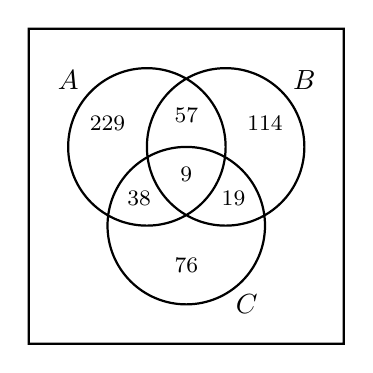
\begin{tikzpicture}
		   \draw[thick] \circleA \circleAlabel \circleB \circleBlabel \circleC \circleClabel \threesetbox;
			 {\footnotesize
		   \draw (0,-.35) node{9} (0,.4) node{57} (-.6,-.65) node{38} (.6,-.65) node{19};
		   \draw (-1,.3) node{229} (1,.3) node{114} (0,-1.5) node{76};% (-1.5,-1.75) node{26};
			 }
		 \end{tikzpicture}

	 \end{center}
		 The region corresponding to multiples of 3 and 5 but not 7 contains 57 elements, and the region corresponding to multiples of 3 and 7 but not 5 contains 38 elements.

		 Thus there are 95 numbers in the requested category.

	\end{solution}


	\end{parts}


	\question[8] How many $9$-bit strings (that is, bit strings of length 9) are there which:
	\begin{parts}
	  \part Start with the sub-string 101? Explain.
	  \begin{solution}
	    $2^6 = 64$.  You have 2 choices for each of the remaining 6 bits.
	  \end{solution}

	  \part Have weight 5 (i.e., contain exactly five 1's) and start with the sub-string 101? Explain.
	  \begin{solution}
	    ${6 \choose 3} = 20$.  You need to choose 3 of the remaining 6 bits to be 1's.
	  \end{solution}

		\part Either start with $101$ or end with $11$ (or both)?  Explain.
			\begin{solution}
				176.  There are 64 strings that start with 101, and another 128 which end with 11 (we choose 1 or 0 for 7 bits, so $2^7$).  However, we count the strings that start with 101 and end with 11 twice - there are $16$ such strings ($2^4$).  So using PIE, we have $64 + 128 - 16 = 176$
			\end{solution}

		\part Have weight 5 and either start with 101 or end with 11 (or both)?  Explain.
		\begin{solution}
		 	51. There are ${6 \choose 3} = 20$ strings of weight 5 which start with 101, and another ${7 \choose 3} = 35$ which end with 11.  We have over counted again - there are weight 5 strings which both start with 101 and end with 11, in fact ${4 \choose 1} = 4$ of them.  So all together we have $20 + 35 - 4 = 51$ strings.
		\end{solution}
	\end{parts}



	\question[8] Gridtown USA, besides having excellent donut shops, is known for its precisely laid out grid of streets and avenues.  Streets run east-west, and avenues north-south, for the entire stretch of the town, never curving and never interrupted by parks or schools or the like.

	Suppose you live on the corner of 3rd and 3rd and work on the corner of 12th and 12th.  Thus you must travel 18 blocks to get to work as quickly as possible.

	\begin{parts}
	\part How many different routes can you take to work, assuming you want to get there as quickly as possible?  Explain.
	\begin{solution}
	  ${18 \choose 9}$ since you must choose 9 of the 18 blocks to travel east.
	\end{solution}

	\part Now suppose you want to stop and get a donut on the way to work, from your favorite donut shop on the corner of 10th ave and 8th st.  How many routes to work, stopping at the donut shop, can you take (again, ensuring the shortest possible route)?  Explain.
	\begin{solution}
	  The donut shop is 12 blocks away, 5 one way, 7 the other.  So to get from home to the donut shop, there are ${12 \choose 7}$ routes (or equivalently, ${12 \choose 5}$).  Then from the donut shop to work, you need to travel 6 more blocks, 2 on way and 4 the other.  So there are ${6 \choose 2}$ (or ${6 \choose 4}$) routes from the donut shop to work.

	  For each of the ways to the donut shop, there are so many ways to work, so the multiplicative principle says the total number of ways from home to work via the donut shop is
	  \[{12 \choose 7}{6 \choose 2}\]
	\end{solution}

	\part Disaster Strikes Gridtown: there is a pothole on 4th ave between 5th st and 6th st.  How many routes to work can you take avoiding that unsightly (and dangerous) stretch of road? Explain.
	\begin{solution}
	  Routes to work that hit the pothole: ${3 \choose 1}1{14 \choose 8}$.

	  There for the number of routes to work which {\em avoid} the pothole are
	  \[{18 \choose 9} - {3 \choose 1}{14 \choose 8}\]
	\end{solution}

	\part The pothole has been repaired (phew) and a new donut shop has opened on the corner of 4th ave and 5th st. How many routes to work drive by one or the other (or both) donut shops?  Hint: the donut shops serve PIE.
	\begin{solution}
	  The routes to work past the donut shop at (4,5): ${3\choose 1}{15 \choose 8}$.  The routes to work past the donut shop at (10,8): ${12 \choose 7}{6 \choose 2}$.  The routes to work past both: ${3\choose 1}{9 \choose 6}{6 \choose 2}$.  So all together, using PIE:
		\[{3\choose 1}{15 \choose 8} + {12 \choose 7}{6 \choose 2} - {3\choose 1}{9 \choose 6}{6 \choose 2}\]
	\end{solution}
	\end{parts}







\end{questions}




\end{document}
